\documentclass{article}

% if you need to pass options to natbib, use, e.g.:
%     \PassOptionsToPackage{numbers, compress}{natbib}
% before loading neurips_2019

% ready for submission
% \usepackage{neurips_2019}

% to compile a preprint version, e.g., for submission to arXiv, add add the
% [preprint] option:
     \usepackage[preprint]{neurips_2019}

% to compile a camera-ready version, add the [final] option, e.g.:
%     \usepackage[final]{neurips_2019}

% to avoid loading the natbib package, add option nonatbib:
%     \usepackage[nonatbib]{neurips_2019}

\usepackage[utf8]{inputenc} % allow utf-8 input
\usepackage[T1]{fontenc}    % use 8-bit T1 fonts
\usepackage{hyperref}       % hyperlinks
\usepackage{url}            % simple URL typesetting
\usepackage{booktabs}       % professional-quality tables
\usepackage{amsfonts}       % blackboard math symbols
\usepackage{nicefrac}       % compact symbols for 1/2, etc.
\usepackage{microtype}      % microtypography

% Not part of the offical NeurIPS template
\usepackage{censor}
\usepackage{amssymb}
\usepackage{amsthm}
\usepackage{mathtools}
\usepackage{caption}
\usepackage{subcaption}
\usepackage{caption}
\usepackage{csquotes}
\usepackage{layouts}
\usepackage{float}
\usepackage{todonotes}
\usepackage{enumitem}

% Algorithms
\usepackage{algorithm}
\usepackage[noend]{algpseudocode}
\algnewcommand{\Let}[2]{\State #1 $\gets$ #2}
\algrenewcommand\Call[2]{\textproc{#1}(#2)}

% Kabel Tables
\usepackage{multirow}
\usepackage{tabu}

\title{Neural Arithmetic Units}

% The \author macro works with any number of authors. There are two commands
% used to separate the names and addresses of multiple authors: \And and \AND.
%
% Using \And between authors leaves it to LaTeX to determine where to break the
% lines. Using \AND forces a line break at that point. So, if LaTeX puts 3 of 4
% authors names on the first line, and the last on the second line, try using
% \AND instead of \And before the third author name.

\author{%
  Andreas Madsen$^{\dag\ddag}$ \\
  \texttt{amwebdk@gmail.com}
  \AND
  Alexander Rosenberg Johansen$^{\dag}$ \\
  \texttt{aler@dtu.dk} \\
  \AND
  Who else? \\
  \\
$^\dag$Technical University of Denmark \quad
$^\ddag$Computationally Demanding
}

\begin{document}
\StopCensoring % NOTE, remove for peer-review to ensure anonymity.

\maketitle

\begin{abstract}
%What’s the domain?
Exact addition, subtraction, multiplication and division present a unique challenge for machine learning models.
%What’s the issue?
Neural networks can approximate complex functions by learning from labeled data.
However, when extrapolating to out-of-distribution samples on arithmetic operations neural networks often fail to learn the underlying logic, which can be the limiting factor for application such as comparing, counting and inferring physical models.
%What’s your contribution?
Our proposed Neural Addition Unit (NAU) and Neural Multiplication Unit (NMU) rely on constrained weights to learn rules and extrapolate well beyond the training distribution.
%We propose a plug-and-play differentiable neural unit that can be trained using stochastic gradient descent to learn addition, subtraction and multiplication between units of a hidden layer.
%Why is it novel?
%What’s interesting about it?
The proposed NAU and NMU are inspired by the underlying arithmetic units of the Neural Arithmetic Logic Unit (NALU).
The NAU learns addition and subtraction through a linear layer of regularized and constrained weights.
The NMU learns multiplication through an accumulative product of the input using gating with an identity function to mask out unwanted elements.
%How does it perform?
Through analytic and empirical analysis we justify how the NAU and NMU improve over the Neural Arithmetic Logic Unit (NALU), a linear regression model and a ReLU based multi-layer perceptron (MLP).
Our NAU and NMU have fewer parameters, converges more consistently, learns faster and have more meaningful discrete values than the NALU and its underlying units.
\end{abstract}

\section{Introduction}
When studying intelligence, insects, reptiles, and humans have been found to possess neurons with the capacity to hold integers, real numbers, and perform arithmetic operations \cite{nieder-neuronal-number,rugani-arithmetic-chicks,gallistel-numbers-in-brain}.
In our quest to mimic intelligence we have put much faith in neural networks, which in turn has provided unparalleled and often superhuman performance in tasks requiring high cognitive abilities \cite{natureGo,bert,openai-learning-dexterous}.
However, when using neural networks to learn simple arithmetic problems, such as counting, multiplication, or comparison they systematically fail to extrapolate onto unseen ranges \cite{stillNotSystematic,suzgun2019evaluating,trask-nalu}.
The absence of inductive bias makes it difficult for neural networks to extrapolate well on arithmetic tasks as they lack the underlying logic to represent the required operations.

We would like to achieve a neural network component that can take an arbitrary hidden input, learn to select the appropriate elements, and apply the desired arithmetic operation.
A recent attempt to achieve this goal is the Neural Arithmetic Logic Unit (NALU), by \citet{trask-nalu}.

The NALU consists of two sub-units: the $\text{NAC}_{+}$ for addition/subtraction and the $\text{NAC}_{\bullet}$ for multiplication/division.
The sub-units are softly gated using a sigmoid function in order to exclusively select one of the sub-units.
However, we find that the soft gating mechanism and the $\text{NAC}_{\bullet}$ are fragile and hard learn.

In this paper, we analyze and improve upon the $\text{NAC}_{+}$ and $\text{NAC}_{\bullet}$ with respect to addition, subtraction, and multiplication.
Our proposed improvements, namely the Neural Addition Unit (NAU) and Neural Multiplication Unit (NMU), are more theoretically founded and improves performance regarding stability, speed of convergence, and interpretability of results.
Most importantly, the NMU can support a large hidden input-size.

The improvements, based on a theoretical analysis of the NALU and its components, are achieved by a simplification of the parameter matrix for a better gradient signal, a sparsity regularizer, and a new multiplication unit that can be optimally initialized and supports both negative and small numbers.
The NMU does not support division.
However, we find that the $\text{NAC}_{\bullet}$ in practice also only supports multiplication and cannot learn division (for theoretical findings on why division is hard to learn, see section \ref{sssec:nac-mul}).

To analyze the impact of each improvement in the NMU by introducing several variants of the $\text{NAC}_{\bullet}$.
We find that, allowing division makes optimization for multiplication harder, linear and regularized weights improve convergence, and that the NMU style of multiplication is critical when increasing the hidden size.

Furthermore, we improve upon existing benchmarks in \citet{trask-nalu} by expanding the ``simple function task'', using a multiplicative variant of ``MNIST Counting and Arithmetic Tasks'', and use an improved success-criterion \citet{maep-madsen-johansen-2019}.
A success-criterion is important because the arithmetic layers are solving a logical problem.
We propose the MNIST multiplication variant as we want to test the NMU's and $\text{NAC}_{\bullet}$'s ability to learn from real data.
%Hence, the solution found is either correct or wrong.
%To test this we propose using a success-criteria to evaluate model performance.
%A success-criterion enables measuring sensitivity to the initialization seed as well as the number of iterations until convergence.

\begin{figure}[t]
\centering
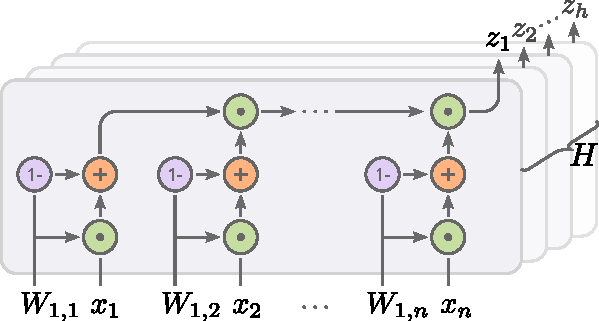
\includegraphics[scale=0.7]{graphics/nmu.pdf}
\caption{Visualization of NMU for a single output scalar $z_1$, this construction repeats for every element in the output vector $\mathbf{z}$.}
\end{figure}

\subsection{Learning a 10 parameter function}
Consider the static function $t = (x_1 + x_2) \cdot (x_1 + x_2 + x_3 + x_4)$ for $x \in \mathbb{R}^4$. To illustrate the ability of $\mathrm{NAC}_{\bullet}$, NALU, and our proposed NMU, we conduct 100 experiemnts for each model, where we attempt to fit this function. Table \ref{tab:very-simple-function-results} show that NMU has a higher success rate and converges faster.
%When inspecting the $6\%$ that did not converge, we found the issue to be underflow when $w = 0$ in the multiplication layer.
\begin{table}[!h]

\caption{\label{tab:very-simple-function-results}Shows the success-rate, at what global step the model converged at, and the sparsity error for all weight matrices, with 95\% confidence interval. Best result is highlighed.}
\centering
\begin{tabular}{crllll}
\toprule
\multicolumn{1}{c}{Op} & \multicolumn{1}{c}{Model} & \multicolumn{1}{c}{Success} & \multicolumn{2}{c}{Solved at} & \multicolumn{1}{c}{Sparsity error} \\
\cmidrule(l{3pt}r{3pt}){1-1} \cmidrule(l{3pt}r{3pt}){2-2} \cmidrule(l{3pt}r{3pt}){3-3} \cmidrule(l{3pt}r{3pt}){4-5} \cmidrule(l{3pt}r{3pt}){6-6}
 &  & Rate & Median & Mean & Mean\\
\midrule
 & $\mathrm{NAC}_{\bullet}$ & $13\% {~}^{+8\%}_{-5\%}$ & $5.5 \cdot 10^{4}$ & $5.9 \cdot 10^{4} {~}^{+7.8 \cdot 10^{3}}_{-6.6 \cdot 10^{3}}$ & $7.5 \cdot 10^{-6} {~}^{+2.0 \cdot 10^{-6}}_{-2.0 \cdot 10^{-6}}$\\

 & NALU & $26\% {~}^{+9\%}_{-8\%}$ & $7.0 \cdot 10^{4}$ & $7.8 \cdot 10^{4} {~}^{+6.2 \cdot 10^{3}}_{-8.6 \cdot 10^{3}}$ & $9.2 \cdot 10^{-6} {~}^{+1.7 \cdot 10^{-6}}_{-1.7 \cdot 10^{-6}}$\\

\multirow{-3}{*}{\centering\arraybackslash $\bm{\times}$} & NMU & $\mathbf{94\%} {~}^{+3\%}_{-6\%}$ & $\mathbf{1.4 \cdot 10^{4}}$ & $\mathbf{1.4 \cdot 10^{4}} {~}^{+2.2 \cdot 10^{2}}_{-2.1 \cdot 10^{2}}$ & $\mathbf{2.6 \cdot 10^{-8}} {~}^{+6.4 \cdot 10^{-9}}_{-6.4 \cdot 10^{-9}}$\\
\bottomrule
\end{tabular}
\end{table}


\section{Improving NAC and NALU}

The NALU from \cite{trask-nalu} is a neural unit capable of doing either exact addition or multiplication, controlled by a sigmoid-gating-mechanism. The addition part is trivial, as this is just a matrix multiplication $\mathbf{a} = \mathbf{W}\mathbf{x}$. The only special part is that the weight matrix $\mathbf{W}$ is constrained to be between $-1$ and $1$. This this done using a $\mathbf{W} = \mathrm{tahn}({\hat{\mathbf{W}}}) \sigma({\hat{\mathbf{M}}})$ construction. Meaning that the weight matrix $\mathbf{W}$ is not trained directly, but computed from two auxiliary weight matrices. The core idea is that $\hat{\mathbf{W}}$ controls the sign and $\hat{\mathbf{M}}$ controls if the weight is zero. One of their core claims, is that this weight matrix construction have a sparse bias, which improves extrapolation for cases where a sparse weight is part of the underlying model.

For the multiplication, an exponential-log transformation is used in order to do exact multiplication (within $\epsilon$ precision) using a matrix multiplication, $\mathbf{m} = \exp(\mathbf{W} \log(|\mathbf{x}| + \epsilon))$.

The addition unit (originally named NAC), and the multiplication unit are in themselves theoretically applicable in any neural network as well as being differentiable. The NALU, then combines them using a sigmoid-gating-mechanism\footnote{The lack of bias term is not a typo. Our preliminary investigations suggests that this is a hack to increase extrapolation of the gate. However in this paper the focus is only arithmetic operators themself.} $\mathbf{g} = \sigma(\mathbf{G} \mathbf{x})$ that chooses softly between addition and multiplication $\mathbf{z} = \mathbf{g} \odot \mathbf{a} + (1 - \mathbf{g}) \odot \mathbf{m}$.

In terms of the theory, the Original NALU paper \cite{trask-nalu} does not discuss anything more than mentioned so-far in this paper. To aid discussion of why this particular construction problematic, and also suggests improvements which will be empirically validated later, the NAC and its multiplication variant is re-formulated using scalar notation.

\begin{equation}
\begin{aligned}
&W_{h_\ell, h_{\ell-1}} = \tanh(\hat{W}_{h_\ell, h_{\ell-1}}) \sigma(\hat{M}_{h_\ell, h_{\ell-1}}) \\
\textrm{NAC}_+:\ &z_{h_\ell} = \sum_{h_{\ell-1}=1}^{H_{\ell-1}} W_{h_{\ell}, h_{\ell-1}} z_{h_{\ell-1}} \\
\textrm{NAC}_\bullet:\ &z_{h_\ell} = \exp\left(\sum_{h_{\ell-1}=1}^{H_{\ell-1}} W_{h_{\ell}, h_{\ell-1}} \log(|z_{h_{\ell-1}}| + \epsilon) \right)
\end{aligned}
\end{equation}

\subsection{Weight matrix construction}

The weight matrix constructions $\mathrm{tahn}({\hat{\mathbf{W}}}) \sigma({\hat{\mathbf{M}}})$ have a few issues worth mentioning. First, the loss gradient with respect to the weight matrices, can without loss of generality, easily be derived to:

\begin{equation}
\begin{aligned}
\frac{\partial \mathcal{L}}{\partial \hat{W}_{h_{\ell-1},h_\ell}} &= \frac{\partial \mathcal{L}}{\partial W_{h_{\ell-1},h_\ell}} (1 - \tanh^2(\hat{W}_{h_{\ell-1},h_\ell})) \sigma(\hat{M}_{h_{\ell-1},h_\ell}) \\
\frac{\partial \mathcal{L}}{\partial \hat{M}_{h_{\ell-1},h_\ell}} &= \frac{\partial \mathcal{L}}{\partial W_{h_{\ell-1},h_\ell}} \tanh(\hat{W}_{h_{\ell-1},h_\ell}) \sigma(\hat{M}_{h_{\ell-1},h_\ell}) (1 - \sigma(\hat{M}_{h_{\ell-1},h_\ell}))
\end{aligned}
\end{equation}

This reveals that this construction is particularly problematic, as $E[\mathrm{tahn}(\hat{W}_{h_{\ell-1},h_\ell})] = 0$ when $E[\hat{W}_{h_{\ell-1},h_\ell}] = 0$. Initializing $\hat{W}_{h_{\ell-1},h_\ell}$ to have zero expectation, is not just common choice but necessary in order to achieve $E[W_{h_{\ell-1},h_\ell}] = 0$, which is necessary to get desired property $E[z_{h_\ell}] = 0$ in linear units such as as the NAC \cite{glorot-initialization}.

The NALU \cite{trask-nalu} paper also claims that this weight matrix construction, creates a bias for $\{-1, 0, 1\}$. However, they provide no empirically or theoretical evidence to support that. In our own empirical investigation as seen in the experiments section, we also find no support for that claim.

To improve on both of these failings, we propose a simple clamped linear construction instead, that is regularize to have the desired bias of $\{-1, 0, 1\}$ and have gradient outside of $[-1, 1]$.

\begin{equation}
\begin{aligned}
&W_{h_{\ell-1},h_\ell} = \min(\max(\hat{W}_{h_{\ell-1},h_\ell}, -1), 1), \\
&\mathcal{R}_{\ell,\mathrm{bias}} = \frac{1}{H_\ell + H_{\ell-1}} \sum_{h_\ell=1}^{H_\ell} \sum_{h_{\ell-1}=1}^{H_{\ell-1}} \hat{W}_{h_{\ell-1},h_\ell}^2 (1 - |\hat{W}_{h_{\ell-1},h_\ell}|)^2 \\
&\mathcal{R}_{\ell,\mathrm{oob}} = \frac{1}{H_\ell + H_{\ell-1}} \sum_{h_\ell=1}^{H_\ell} \sum_{h_{\ell-1}=1}^{H_{\ell-1}} \max(|\hat{W}_{h_{\ell-1},h_\ell}| - 1, 0)^2 \\
\textrm{NAU}:\ &z_{h_\ell} = \sum_{h_{\ell-1}=1}^{H_{\ell-1}} W_{h_{\ell}, h_{\ell-1}} z_{h_{\ell-1}} \\\end{aligned}
\end{equation}

Note that while the bias regularizer $\mathcal{R}_{\ell,\mathrm{bias}}$ also regularize $\hat{W}_{h_{\ell-1},h_\ell}$ to not be outside of $[-1, 1]$, one may choose a small regularization constant for this, or scale it up gradually as done in the experiments later. However, $\mathcal{R}_{\ell,\mathrm{oob}}$ should always be present as it is never desired to have $\hat{W}_{h_{\ell-1},h_\ell} \not\in [-1, 1]$.

\subsection{Multiplication unit}

The multiplication unit has its own issues. It should be easy to see that when $|z_{h_{\ell-1}}|$ is near zero and when $\hat{W}_{h_{\ell-1},h_\ell}$ is near $-1$ the $z_{h_\ell}$ value explodes. However, the issue extends beyond a weight near $-1$ as is revealed in the gradients, especially the backpropergation term $\frac{\partial z_{h_\ell}}{\partial z_{h_{\ell-1}}}$:

\begin{equation}
\begin{aligned}
\frac{\partial \mathcal{L}}{\partial W_{h_{\ell}, h_{\ell - 1}}} &= \frac{\partial \mathcal{L}}{\partial z_{h_\ell}} \frac{\partial z_{h_\ell}}{\partial W_{h_{\ell}, h_{\ell - 1}}} = \frac{\partial \mathcal{L}}{\partial z_{h_\ell}} z_{h_\ell} \log(|z_{h_{\ell-1}}| + \epsilon) \\
\frac{\partial \mathcal{L}}{\partial z_{h_{\ell-1}}} &= \sum_{h_\ell = 1}^{H_\ell} \frac{\partial \mathcal{L}}{\partial z_{h_\ell}} \frac{\partial z_{h_\ell}}{\partial z_{h_{\ell-1}}} = \sum_{h_\ell = 1}^{H_\ell} \frac{\partial \mathcal{L}}{\partial z_{h_\ell}} z_{h_\ell} W_{h_\ell, h_{\ell-1}} \frac{\mathrm{sign}(z_{h_{\ell-1}})}{|z_{h_{\ell-1}}| + \epsilon}
\end{aligned}
\end{equation}

In should be clear from $\frac{\mathrm{sign}(z_{h_{\ell-1}})}{|z_{h_{\ell-1}}| + \epsilon}$ that for $z_{h_{\ell-1}}$ near zero, the backpropagation term will not only explode, but can oscillate between a large postive value and large negative value, which is very problematic in optimization \cite{adam-optimization}. This issue does not only exists for $|z_{h_{\ell-1}}| < \epsilon$, which may have a small probability if $z_{h_{\ell-1}}$ has a wide distribution. But is can also be an issue for values outside of this interval as seen in figure \ref{fig:nac-mul-eps-issue}.

\begin{figure}[H]
\centering
\begin{subfigure}{.33\textwidth}
  \centering
  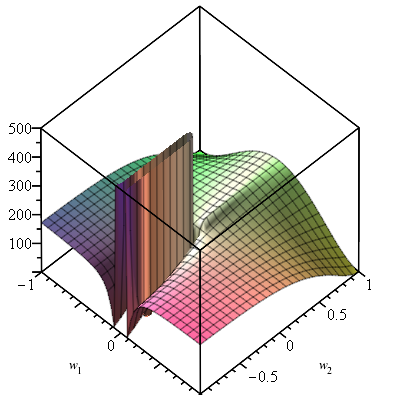
\includegraphics[width=\linewidth]{graphics/nac-mul-eps-1em7.png}
  \caption{$\epsilon = 10^{-7}$}
\end{subfigure}%
\begin{subfigure}{.33\textwidth}
  \centering
  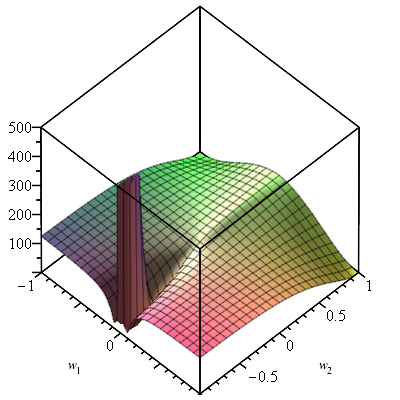
\includegraphics[width=\linewidth]{graphics/nac-mul-eps-1em1.png}
  \caption{$\epsilon = 0.1$}
\end{subfigure}
\begin{subfigure}{.33\textwidth}
  \centering
  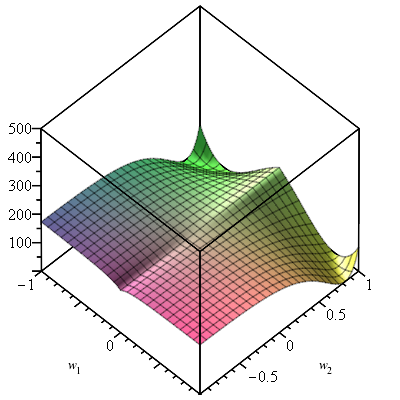
\includegraphics[width=\linewidth]{graphics/nac-mul-eps-1.png}
  \caption{$\epsilon = 1$}
\end{subfigure}
\caption{RMS loss curvature for a $\mathrm{NAC}_{+}$ layer followed by a $\mathrm{NAC}_{\bullet}$ layer. The weight matrices constrained are to $\mathbf{W}_1 = \left[\protect\begin{smallmatrix}
w_1 & w_1 & 0 & 0 \\
w_1 & w_1 & w_1 & w_1
\protect\end{smallmatrix}\right]$, $\mathbf{W}_2 = \left[\protect\begin{smallmatrix}
w_2 & w_2
\protect\end{smallmatrix}\right]$. The problem is $x = \left(1, 1.2, 1.8, 2\right), t = 11.25$. Desired solution is $w_1 = w_2 = 1$, although this problem have additional undesired solutions.}
\label{fig:nac-mul-eps-issue}
\end{figure}

These observations are particular problematic when considering that $E[z_{h_{\ell-1}}] = 0$ is a desired property when initializing \cite{glorot-initialization}. An alternative multiplication operator must thus be able to not explode for $z_{h_{\ell-1}}$ near zero. To that end we propose a new neural multplication units (NMU): 

\begin{equation}
\begin{aligned}
&W_{h_{\ell-1},h_\ell} = \min(\max(\hat{W}_{h_{\ell-1},h_\ell}, 0), 1), \\
&\mathcal{R}_{\ell,\mathrm{bias}} = \frac{1}{H_\ell + H_{\ell-1}} \sum_{h_\ell=1}^{H_\ell} \sum_{h_{\ell-1}=1}^{H_{\ell-1}} \hat{W}_{h_{\ell-1},h_\ell}^2 (1 - \hat{W}_{h_{\ell-1},h_\ell})^2 \\
&\mathcal{R}_{\ell,\mathrm{oob}} = \frac{1}{H_\ell + H_{\ell-1}} \sum_{h_\ell=1}^{H_\ell} \sum_{h_{\ell-1}=1}^{H_{\ell-1}} \max\left(\left|\hat{W}_{h_{\ell-1},h_\ell} - \frac{1}{2}\right| - \frac{1}{2}, 0\right)^2 \\
\textrm{NMU}:\ &z_{h_\ell} = \prod_{h_{\ell-1}=1}^{H_{\ell-1}} \left(W_{h_{\ell-1},h_\ell} z_{h_{\ell-1}} + 1 - W_{h_{\ell-1},h_\ell} \right)
\end{aligned}
\end{equation}

This units does not support division. But supporting division is likely infeasible if $z_{h_{\ell-1}}$ near zero should not cause explosions. The NALU paper also shows that division doesn't work well for their unit, hence very little is lost here \cite{trask-nalu}. On the other hand, this unit construction understand the difference between a negative and a positive $z_{h_{\ell-1}}$ values, which should be considered an added bonus,as this allows extrapolations into the negative input range.

The gradients weight gradient and backpropagation term of the NMU are:
\begin{equation}
\begin{aligned}
\frac{\partial \mathcal{L}}{\partial W_{h_{\ell}, h_{\ell - 1}}} &= \frac{\partial \mathcal{L}}{\partial z_{h_\ell}} \frac{\partial z_{h_\ell}}{\partial W_{h_{\ell}, h_{\ell - 1}}} = \frac{\partial \mathcal{L}}{\partial z_{h_\ell}} \frac{z_{h_\ell}}{W_{h_{\ell-1},h_\ell} z_{h_{\ell-1}} + 1 - W_{h_{\ell-1},h_\ell}} \left(z_{h_{\ell-1}} - 1\right) \\
\frac{\partial \mathcal{L}}{\partial z_{h_{\ell-1}}} &= \sum_{h_\ell = 1}^{H_\ell} \frac{\partial \mathcal{L}}{\partial z_{h_\ell}} \frac{\partial z_{h_\ell}}{\partial z_{h_{\ell-1}}} = \sum_{h_\ell = 1}^{H_\ell} \frac{z_{h_\ell}}{W_{h_{\ell-1},h_\ell} z_{h_{\ell-1}} + 1 - W_{h_{\ell-1},h_\ell}} W_{h_{\ell-1},h_\ell}
\end{aligned}
\end{equation}

These is much more well-behaved. Note also that the fraction does not explode for $z_{h_{\ell-1}}$ close to zero, as the denominator simply cancels out a term in $z_{h_\ell}$.

\begin{figure}[H]
\centering
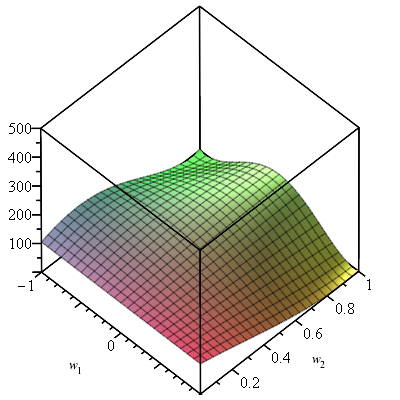
\includegraphics[width=0.33\linewidth]{graphics/nac-mul-nmu.png}
\caption{RMS loss curvature (without regularization) for a $\mathrm{NAC}_{+}$ layer followed by an $\mathrm{NMU}$ layer. Otherwise, the setup is identical to that in Figure \ref{fig:nac-mul-eps-issue}.}
\end{figure}

\subsection{Moments and initialization for addition}

Initialization is important for fast and consistent convergence. The desired properties are according to Glorot et al. \cite{glorot-initialization}:
\begin{equation}
\begin{aligned}
E[z_{h_\ell}] &= 0 & E\left[\frac{\partial \mathcal{L}}{\partial z_{h_{\ell-1}}}\right] &= 0 \\
Var[z_{h_\ell}] &= Var\left[z_{h_{\ell-1}}\right] &
Var\left[\frac{\partial \mathcal{L}}{\partial z_{h_{\ell-1}}}\right] &= Var\left[\frac{\partial \mathcal{L}}{\partial z_{h_{\ell}}}\right]
\end{aligned}
\end{equation}

The $\mathrm{NAC}_{+}$ layer is trivial, as this is just a linear layer. Thus the result from Glorot et al. ($Var[W_{h_{\ell-1},h_{\ell}}] = \frac{2}{H_{\ell-1} + H_{\ell}}$) can be used \cite{glorot-initialization}.

In the case of the $\mathrm{NAU}$, this condition is easy to satisfy. However, the original $\mathrm{NAC}_{+}$ unit is less trivial as $W_{h_{\ell-1},h_{\ell}}$ is not sampled directly. But assuming that $\hat{W}_{h_\ell, h_{\ell-1}} \sim \mathrm{Uniform}[-r, r]$ and $\hat{M}_{h_\ell, h_{\ell-1}} \sim \mathrm{Uniform}[-r, r]$ then the variance can be derived to be:
\begin{equation}
Var[W_{h_{\ell-1},h_{\ell}}] = \frac{1}{2r} \left(1 - \frac{\tanh(r)}{r}\right) \left(r - \tanh\left(\frac{r}{2}\right)\right)
\end{equation}
One can the solve for $r$, given the desired variance. 

\subsection{Moments and initialization for multiplication}

Using second order multivariate Taylor approximation and some assumptions of uncorrelated stochastic variables, the expectation and variance of the $\mathrm{NAC}_{\bullet}$ layer can be estimated to:
\begin{equation}
\begin{aligned}
f(c_1, c_2) &= \left(1 + c_1 \frac{1}{2} Var[W_{h_\ell, h_{\ell-1}}] \log(|E[z_{h_{\ell-1}}]| + \epsilon)^2\right)^{c_2\ H_{\ell-1}} \\
E[z_{h_\ell}] &\approx f\left(1, 1\right) \\
Var[z_{h_2}] &\approx f\left(4, 1\right) - f\left(1, 2\right) \\
E\left[\frac{\partial \mathcal{L}}{\partial z_{h_{\ell-1}}}\right] &= 0 \\
Var\left[\frac{\partial \mathcal{L}}{\partial z_{h_{\ell-1}}}\right] &\approx Var\left[\frac{\partial \mathcal{L}}{\partial z_{h_{\ell}}}\right] H_{\ell}\ f\left(4, 1\right)\ Var[W_{h_{\ell}, h_{\ell-1}}] \\
&\cdot \left(\frac{1}{\left(|E[z_{h_{\ell-1}}]| + \epsilon\right)^2} + \frac{3}{\left(|E[z_{h_{\ell-1}}]| + \epsilon\right)^4} Var[z_{h_{\ell-1}}]\right)
\end{aligned}
\end{equation}

This is problematic because $E[z_{h_\ell}] \ge 1$, and the variance explodes for $E[z_{h_{\ell-1}}] = 0$ which is normally a desired property.

For our proposed NMU, the expectation and variance can be derived using the same assumptions as before, although no Taylor approximation is required:
\begin{equation}
\begin{aligned}
E[z_{h_\ell}] &\approx \left(\frac{1}{2}\right)^{H_{\ell-1}} \\
E\left[\frac{\partial \mathcal{L}}{\partial z_{h_{\ell-1}}}\right] &\approx 0 \\
Var[z_{h_\ell}] &\approx \left(Var[W_{h_{\ell-1},h_\ell}] + \frac{1}{4}\right)^{H_{\ell-1}} \left(Var[z_{h_{\ell-1}}] + 1\right)^{H_{\ell-1}} - \left(\frac{1}{4}\right)^{H_{\ell-1}} \\
Var\left[\frac{\partial \mathcal{L}}{\partial z_{h_{\ell-1}}}\right] &\approx Var\left[\frac{\partial \mathcal{L}}{\partial z_{h_\ell}}\right] H_\ell \\
& \cdot \left( \left(Var[W_{h_{\ell-1},h_\ell}] + \frac{1}{4}\right)^{H_{\ell-1}} \left(Var[z_{h_{\ell-1}}] + 1\right)^{H_{\ell-1}-1} - \left(\frac{1}{4}\right)^{H_{\ell-1}}\right)
\end{aligned}
\end{equation}

These expectations are much more well behaved. It is properly unlikely to expect that the expectation can become zero, since the identity for multiplication is 1. However, for a large $H_{\ell-1}$ it will be near zero.

The variance is also more well-behaved, but does not provide a input-independent initialization strategy. We propose initializing with $Var[W_{h_{\ell-1},h_\ell}] = \frac{1}{4}$, as this is the solution to $Var[z_{h_\ell}] = Var[z_{h_{\ell-1}}]$ assuming $Var[z_{h_{\ell-1}}] = 1$ and a large $H_{\ell-1}$. However, feel free to compute more exact solutions.


\section{Experimental results}
\label{sec:experiments}

\subsection{Arithmetic datasets}
\label{sec:arithmetic-dataset}

The arithmetic dataset is a replica of the "simple function task" as shown in \cite{trask-nalu}.
The goal is to sum two random subsets of a vector and perform a arithmetic operation as defined below
\begin{equation}
t = \sum_{i = s_{1,\mathrm{start}}}^{s_{1,\mathrm{end}}} x_i \circ \sum_{i = s_{2,\mathrm{start}}}^{s_{2,\mathrm{end}}} x_i \quad \text{where } \mathbf{x} \in \mathbb{R}^n, x_i \sim \mathrm{Uniform}[r_{\mathrm{lower}}, r_{\mathrm{upper}}], \circ \in \{+, -, \times\}
\label{eq:arithmetic-problem}
\end{equation}
where $n$ (default $100$), $U[r_{\mathrm{lower}}, r_{\mathrm{upper}}]$ (interpolation default is $U[1,2]$ and extrapolation default is $U[2,6]$), the subset size (default 25\%), and subset overlap (default 50\%) are parameters that we use to assess learning capability (see details in appendix \ref{sec:appendix:simple-function-task:data-generation} and the effect of varying the parameters in appendix \ref{sec:appendix-simple-function-task:dataset-parameter-effect}).

\subsubsection{Model evaluation}
The goal is to achieve a solution that is acceptably close to a perfect solution. To evaluate if a model instance solves the task consistently we compare the MSE to a nearly-perfect solution on the extrapolation range over multiple seeds. If $\mathbf{W}_1, \mathbf{W}_2$ defines the weights of the fitted model, and $\mathbf{W}_1^\epsilon$ is nearly-perfect and $\mathbf{W}_2^*$ is perfect (example in equation \ref{eq:nearly-perfect-solution-example}), the success criteria is $\mathcal{L}_{\mathbf{W}_1, \mathbf{W}_2} < \mathcal{L}_{\mathbf{W}_1^\epsilon, \mathbf{W}_2^*}$, measured on the extrapolation error, for $\epsilon = 10^{-5}$.
\begin{equation}
    \mathbf{W}_1^\epsilon = \begin{bmatrix}
    1 - \epsilon & 1 - \epsilon & 0 + \epsilon & 0 + \epsilon \\
    1 - \epsilon & 1 - \epsilon & 1 - \epsilon & 1 - \epsilon
    \end{bmatrix}, \mathbf{W}_2^* = \begin{bmatrix}
    1 & 1
    \end{bmatrix}
    \label{eq:nearly-perfect-solution-example}
\end{equation}
To measure speed of convergence the first iteration for which $\mathcal{L}_{\mathbf{W}_1, \mathbf{W}_2} < \mathcal{L}_{\mathbf{W}_1^\epsilon, \mathbf{W}_2^*}$ is reported with a 95\% confidence interval. Only models that managed to solve the task are included.

We assume an approximate discrete solution with parameters close to $\{-1, 0, 1\}$ is important for inferring exact arithmetic operations.
To measure the sparsity we introduce a sparsity error (defined in equation \ref{eq:sparsity-error}).
Similar to the convergence metric we only considered model instances that did solve the task and report the 95\% confidence interval.
\begin{equation}
E_\mathrm{sparsity} = \max_{h_{\ell-1}, h_{\ell}} \min(|W_{h_{\ell-1},h_\ell}|, |1 - |W_{h_{\ell-1},h_\ell}||)
\label{eq:sparsity-error}
\end{equation}

We evaluate each metric every $1000$ iterations on the test set that uses the extrapolation range, and choose the best iteration based on the validation dataset that uses the interpolation range.

\subsubsection{Arithmetic operation comparison}
We compare models on different arithmetic operation $\circ \in \{+, -, \times\}$. The multiplication models, NMU and $\mathrm{NAC}_{\bullet}$, have an addition layer first, either NAU or $\mathrm{NAC}_{+}$, followed by a multiplication layer. The addition models are just two layers of the same unit. Finally, the NALU model consists of two NALU layers. See explicit definitions in appendix \ref{sec:appendix:comparison-all-models}.

Each experiment is trained for $5 \cdot 10^6$ iterations (details in appendix \ref{sec:appendix:comparison-all-models}). Results are presented in table \ref{tab:function-task-static-defaults}. For multiplication, the NMU succeeds more often and converges faster. For addition and subtraction, the NAU model converges faster, given the median, and has a sparser solution. A larger comparison is in appendix \ref{sec:appendix:comparison-all-models} and an ablation study is in appendix \ref{sec:appendix:ablation-study}.

\begin{table}[!h]

\caption{\label{tab:function-task-static-defaults}Shows the success-rate for $\mathcal{L}_{\mathbf{W}_1, \mathbf{W}_2} < \mathcal{L}_{\mathbf{W}_1^\epsilon, \mathbf{W}_2^*}$, at what global step the model converged at, and the sparsity error for all weight matrices.}
\centering
\begin{tabular}{crllll}
\toprule
\multicolumn{1}{c}{Op} & \multicolumn{1}{c}{Model} & \multicolumn{1}{c}{Success} & \multicolumn{2}{c}{Solved at} & \multicolumn{1}{c}{Sparsity error} \\
\cmidrule(l{3pt}r{3pt}){1-1} \cmidrule(l{3pt}r{3pt}){2-2} \cmidrule(l{3pt}r{3pt}){3-3} \cmidrule(l{3pt}r{3pt}){4-5} \cmidrule(l{3pt}r{3pt}){6-6}
 &  & Rate & Median & Mean & Mean\\
\midrule
 & $\mathrm{NAC}_{\bullet}$ & $30\%$ & $2.5 \cdot 10^{6}$ & $2.5 \cdot 10^{6} \pm 1.5 \cdot 10^{6}$ & $\mathbf{3.9 \cdot 10^{-4} \pm 9.4 \cdot 10^{-4}}$\\

 & Linear & $0\%$ & --- & --- & ---\\

 & NALU & $0\%$ & --- & --- & ---\\

\multirow{-4}{*}{\centering\arraybackslash $\bm{\times}$} & NMU & $\mathbf{90\%}$ & $\mathbf{1.4 \cdot 10^{6}}$ & $\mathbf{1.6 \cdot 10^{6} \pm 5.6 \cdot 10^{5}}$ & $1.8 \cdot 10^{-3} \pm 1.1 \cdot 10^{-3}$\\
\cmidrule{1-6}
 & $\mathrm{NAC}_{+}$ & $\mathbf{100\%}$ & $6.0 \cdot 10^{4}$ & $7.1 \cdot 10^{4} \pm 2.4 \cdot 10^{4}$ & $4.8 \cdot 10^{-1} \pm 2.0 \cdot 10^{-2}$\\

 & Linear & $\mathbf{100\%}$ & $4.2 \cdot 10^{4}$ & $\mathbf{4.2 \cdot 10^{4} \pm 1.9 \cdot 10^{3}}$ & $6.1 \cdot 10^{-1} \pm 1.2 \cdot 10^{-1}$\\

 & NALU & $0\%$ & --- & --- & ---\\

\multirow{-4}{*}{\centering\arraybackslash $\bm{+}$} & NAU & $\mathbf{100\%}$ & $\mathbf{1.8 \cdot 10^{4}}$ & $7.0 \cdot 10^{5} \pm 9.2 \cdot 10^{5}$ & $\mathbf{1.7 \cdot 10^{-3} \pm 8.0 \cdot 10^{-4}}$\\
\cmidrule{1-6}
 & $\mathrm{NAC}_{+}$ & $\mathbf{100\%}$ & $8.0 \cdot 10^{3}$ & $1.5 \cdot 10^{6} \pm 1.5 \cdot 10^{6}$ & $4.6 \cdot 10^{-1} \pm 2.9 \cdot 10^{-2}$\\

 & Linear & $\mathbf{100\%}$ & $1.1 \cdot 10^{6}$ & $1.9 \cdot 10^{6} \pm 1.3 \cdot 10^{6}$ & $3.7 \cdot 10^{-1} \pm 1.1 \cdot 10^{-1}$\\

 & NALU & $20\%$ & $3.6 \cdot 10^{6}$ & $3.6 \cdot 10^{6} \pm 1.3 \cdot 10^{7}$ & $4.7 \cdot 10^{-1} \pm 3.3 \cdot 10^{-1}$\\

\multirow{-4}{*}{\centering\arraybackslash $\bm{-}$} & NAU & $\mathbf{100\%}$ & $\mathbf{4.0 \cdot 10^{3}}$ & $\mathbf{4.2 \cdot 10^{3} \pm 3.0 \cdot 10^{2}}$ & $\mathbf{1.9 \cdot 10^{-3} \pm 4.2 \cdot 10^{-4}}$\\
\bottomrule
\end{tabular}
\end{table}


\subsubsection{Evaluating theoretical claims}

To validate our theoretical claim, that the NMU models works better than $NAC_{\bullet}$ for larger $H_{\ell-1}$, we increase the hidden size of the network, thereby adding redundant units. Redundant units are very common neural networks, where the purpose is to fit an unknown function.

Additionally, the NMU model is unlike the $NAC_{\bullet}$ model also capable of understanding inputs that are both negative and positive. To validate this empirically, the training and validation datasets are sampled for $\mathrm{U}[-2,2]$, and then tested on $\mathrm{U}[-6,-2] \cup \mathrm{U}[2,6]$.

Finally, to validate that division and the lack of bias in $NAC_{\bullet}$ are critical issues but that solving these alone are not enough, two additional models compared with. A variant of $\mathrm{NAC}_{\bullet}$ called $\mathrm{NAC}_{\bullet, \sigma}$, that only supports multiplication, by constraining the weights with $W = \sigma(\hat{W})$. And a variant, called $\mathrm{NAC}_{\bullet, \mathrm{NMU}}$, that uses linear weights and bias regularization, identically to that in NMU model.

Figure \ref{fig:simple-function-static-theoreical-claims-experiment} shows that the NMU can both handle a much larger hidden-size, as well as negative inputs, and that solving the division and bias issues alone improves the success rate, but are no enough when the hidden-size is large, as there is no ideal initialization.

\begin{figure}[h]
\centering
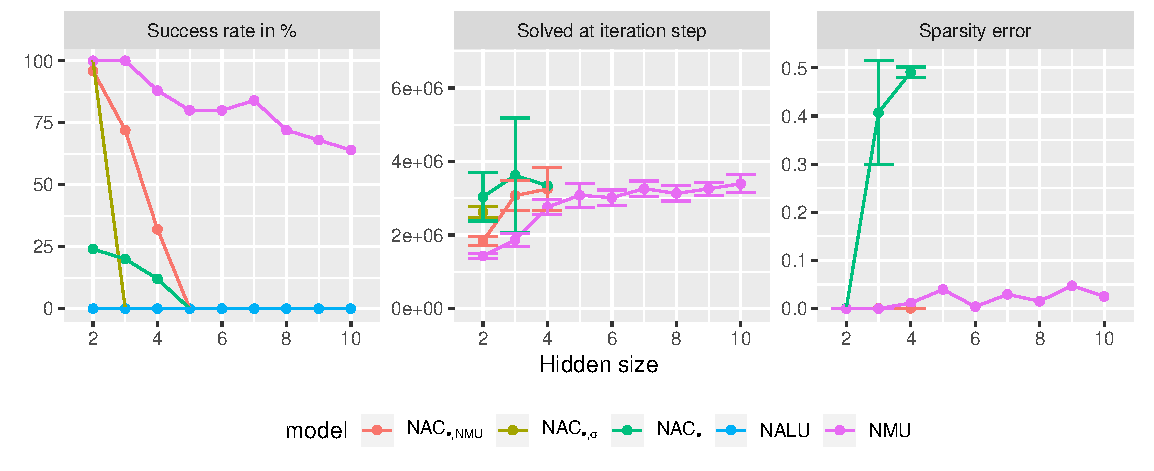
\includegraphics[width=\linewidth,trim={0 1.3cm 0 0},clip]{results/simple_function_static_mul_hidden_size.pdf}
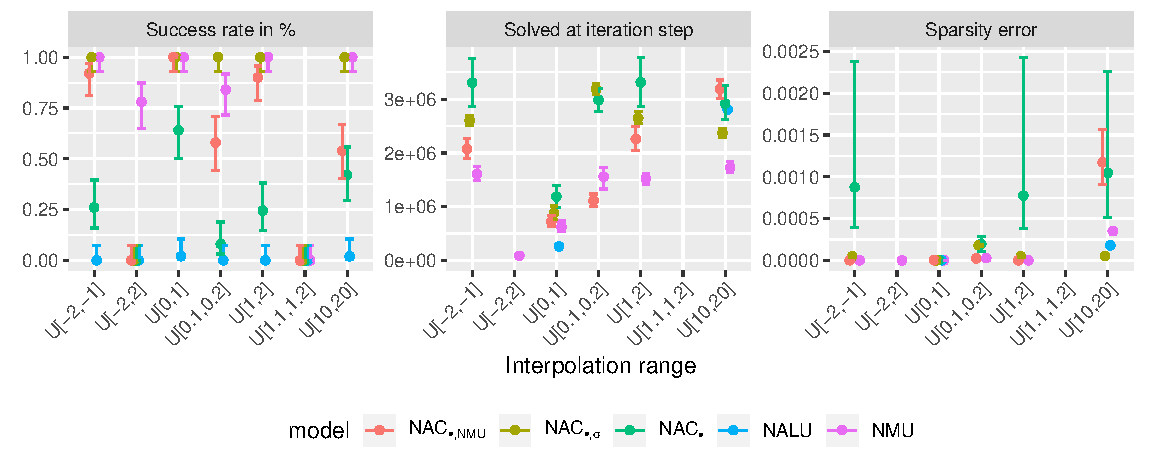
\includegraphics[width=\linewidth,trim={0 0 0 0.809cm},clip]{results/simple_function_static_mul_range.pdf}
\caption{Shows that the NMU can handle a large hidden size, and works when the input contains both positive and negative numbers ($U[-2,-2]$).} 
%\caption{Shows the effect of the dataset parameters. For each interpolation range, the following extrapolation ranges are used: ${\mathrm{U}[-2,2] \rightarrow \mathrm{U}[-6,-2] \cup \mathrm{U}[2,6]}$, ${\mathrm{U}[0,1] \rightarrow \mathrm{U}[1,5]}$, ${\mathrm{U}[0.1,0.2] \rightarrow \mathrm{U}[0.2,2]}$, ${\mathrm{U}[1,2] \rightarrow \mathrm{U}[2,6]}$, ${\mathrm{U}[10, 20] \rightarrow \mathrm{U}[20, 40]}$. The uniform sampling ranges are chosen to test the effect of mean, variance, and sign for optimizing.}
\label{fig:simple-function-static-theoreical-claims-experiment}
\end{figure}

\subsection{Product of sequential MNIST}

To compare how easy it is to backpropergation though the arithmetic layers, the arithmetic layers are applied as a recurrent-unit to a sequence of MNIST digits, where the target is to fit the cumulative product. This task is similar to ``MNIST Counting and Arithmetic Tasks'' in \cite{trask-nalu}\footnote{Also uses the same CNN, \url{https://github.com/pytorch/
examples/tree/master/mnist}.}, but use multiplication rather than addition.. Each model is trained on sequences of length 2, and then tested on sequences of length 20 MNIST digits.

Success of convergence is determined by comparing the MSE of each model, with a baseline model that directly computes the sequential product. If the MSE of each model, is less than the upper 1\% MSE-confidence-interval of the baseline model, then the model is considered successfully converged.

Sparsity and ``solved at iteration step'' is determined as described in experiment \ref{sec:arithmetic-dataset}. The validation set is the last 5000 MNIST digits from the training set, which is used to select the best epoch.

In this experiment we discovered that having an unconstrained ``input-network'' causes the multiplication-units to learn an undesired solution, such as $(0.1 \cdot 81 + 1 - 0.1) = 9$. This solves the problem with a similar success-rate, but not in the intended way. To prevent such solution, we regularize the CNN output with $\mathcal{R}_{\mathrm{z}} = \frac{1}{H_{\ell-1} H_\ell} \sum_{h_\ell}^{H_\ell} \sum_{h_{\ell-1}}^{H_{\ell-1}} (1 - W_{h_{\ell-1},h_\ell}) \cdot (1 - \bar{z}_{h_{\ell-1}})^2$. This regularizer is applied to the NMU and $\mathrm{NAC}_{\bullet,\mathrm{NMU}}$ models. See appendix \ref{sec:appendix:sequential-mnist:ablation} for the results, when this regularizer is not used.

Figure \ref{fig:sequential-mnist-prod-results} shows that the NMU does not hindre learning a more complex neural network. And that it can extrapolate to much longer sequences than what is is trained on.

\begin{figure}[h]
\centering
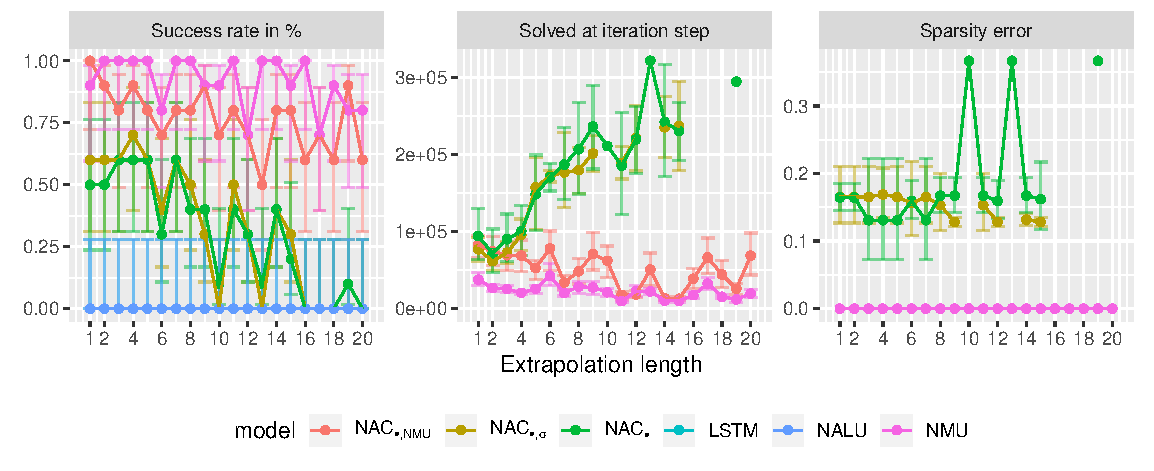
\includegraphics[width=\linewidth,trim={0 0.5cm 0 0},clip]{results/sequential_mnist_prod_long.pdf}
\caption{Shows the ability of each model to backpropergation and extrapolate to larger sequence lengths.} 
\label{fig:sequential-mnist-prod-results}
\end{figure}

\section{Future work}

\begin{itemize}
    \item Lorem Ipsum
\end{itemize}


\section{Conclusion}
By including theoretical considerations, such as initialization, gradients, and sparsity, we have developed a new multiplication unit that outperforms the state-of-the-art models on established extrapolation and sequential tasks. Our model converges more consistently, faster, and to more sparse solutions, than previously proposed models. 

We find that performing division and multiplication concurrently is a hard problem because of division by zero that currently can not be solved. However, when it comes to multiplication, our model is capable of extrapolating in both the negative range and to very small numbers.
%A theoretical disadvantage of our multiplication unit is that it is incapable of division. However, previous publications concur that this is a problematic and generally unsolved area, due to the singularity in division. Thus our proposed model is empirically identical when it comes to division. On the other hand, when it comes to multiplication, our model is capable of extrapolating in both the negative range and to very small numbers.

Finally, when it comes to considering more than just two inputs to the multiplication layer, our model clearly outperforms all previously proposed models as well as variations of previous models that borrow from our model. The ability for a neural layer to consider more than just two inputs, is critical in neural networks where the desired function is unknown.

\subsubsection*{Acknowledgments}

\xblackout{We would like to thank Andrew Trask and the other authors of the NALU paper, for highlighting the importance and challenges of etrapolation in Neural Networks. We would also like to thank the students Raja Shan Zaker Kreen and William Frisch Moller from The Technical University of Denmark, who showed us that the NALU does not converge consistently.}

\bibliographystyle{plainnat}
\bibliography{bibliography}

\newpage
\appendix
\section{Gradient derivatives}
\label{sec:appendix:gradient-derivatives}

\subsection{Weight matrix construction}
\label{sec:appendix:gradient-derivatives:weight-matrix-construction}
For clarity the weight matrix construction is defined using scalar notation
\begin{equation}
W_{h_\ell, h_{\ell-1}} = \tanh(\hat{W}_{h_\ell, h_{\ell-1}}) \sigma(\hat{M}_{h_\ell, h_{\ell-1}})
\end{equation}

The of the loss with respect to $\hat{W}_{h_\ell, h_{\ell-1}}$ and $\hat{M}_{h_\ell, h_{\ell-1}}$ is then straight forward to derive.
\begin{equation}
\begin{aligned}
\frac{\partial\mathcal{L}}{\partial \hat{W}_{h_\ell, h_{\ell-1}}} &= \frac{\partial\mathcal{L}}{\partial W_{h_\ell, h_{\ell-1}}} \frac{\partial W_{h_\ell, h_{\ell-1}}}{\partial \hat{W}_{h_\ell, h_{\ell-1}}} \\
&= \frac{\partial\mathcal{L}}{\partial W_{h_\ell, h_{\ell-1}}} (1 - \tanh^2(\hat{W}_{h_\ell, h_{\ell-1}})) \sigma(\hat{M}_{h_\ell, h_{\ell-1}}) \\
\frac{\partial\mathcal{L}}{\partial \hat{M}_{h_\ell, h_{\ell-1}}} &= \frac{\partial\mathcal{L}}{\partial W_{h_\ell, h_{\ell-1}}} \frac{\partial W_{h_\ell, h_{\ell-1}}}{\partial \hat{M}_{h_\ell, h_{\ell-1}}} \\
&= \frac{\partial\mathcal{L}}{\partial W_{h_\ell, h_{\ell-1}}} \tanh(\hat{W}_{h_\ell, h_{\ell-1}}) \sigma(\hat{M}_{h_\ell, h_{\ell-1}}) (1 - \sigma(\hat{M}_{h_\ell, h_{\ell-1}}))
\end{aligned}
\end{equation}

As seen from this result, one only needs to consider $\frac{\partial\mathcal{L}}{\partial W_{h_\ell, h_{\ell-1}}}$ for $\mathrm{NAC}_{+}$ and $\mathrm{NAC}_{\bullet}$, as the gradient with respect to $\hat{W}_{h_\ell, h_{\ell-1}}$ and $\hat{M}_{h_\ell, h_{\ell-1}}$ is just a multiplication on $\frac{\partial\mathcal{L}}{\partial W_{h_\ell, h_{\ell-1}}}$.

\subsection{Gradient of $\mathrm{NAC}_{\bullet}$}
\label{sec:appendix:gradient-derivatives:gradient-nac-mul}

First the $\textrm{NAC}_\bullet$ is defined using scalar notation.
\begin{equation}
z_{h_\ell} = \exp\left(\sum_{h_{\ell-1}=1}^{H_{\ell-1}} W_{h_{\ell}, h_{\ell-1}} \log(|z_{h_{\ell-1}}| + \epsilon) \right)
\end{equation}

The gradient of the loss with respect to $W_{h_\ell, h_{\ell-1}}$ is straight forward to derive.
\begin{equation}
\begin{aligned}
\frac{\partial z_{h_\ell}}{\partial W_{h_\ell, h_{\ell-1}}} &= \exp\left(\sum_{h'_{\ell-1}=1}^{H_{\ell-1}} W_{h_{\ell}, h'_{\ell-1}} \log(|z_{h'_{\ell-1}}| + \epsilon) \right) \log(|z_{h_{\ell-1}}| + \epsilon) \\
&= z_{h_\ell} \log(|z_{h_{\ell-1}}| + \epsilon)
\end{aligned}
\end{equation}

We now wish to derive the backpropagation term $\delta_{h_\ell} = \frac{\partial \mathcal{L}}{\partial z_{h_\ell}}$, because $z_{h_\ell}$ affects $\{z_{h_{\ell+1}}\}_{h_{\ell+1}=1}^{H_{\ell+1}}$ this becomes:
\begin{equation}
\delta_{h_\ell} = \frac{\partial \mathcal{L}}{\partial z_{h_\ell}} = \sum_{h_{\ell+1}=1}^{H_{\ell+1}} \frac{\partial \mathcal{L}}{\partial z_{h_{\ell+1}}} \frac{\partial z_{h_{\ell+1}}}{\partial z_{h_\ell}} = \sum_{h_{\ell+1}=1}^{H_{\ell+1}} \delta_{h_{\ell+1}} \frac{\partial z_{h_{\ell+1}}}{\partial z_{h_\ell}}
\end{equation}

To make it easier to derive $\frac{\partial z_{h_{\ell+1}}}{\partial z_{h_\ell}}$ we re-express the $z_{h_\ell}$ as $z_{h_{\ell+1}}$.
\begin{equation}
z_{h_{\ell+1}} = \exp\left(\sum_{h_{\ell}=1}^{H_{\ell}} W_{h_{\ell+1}, h_{\ell}} \log(|z_{h_{\ell}}| + \epsilon) \right)
\end{equation}

The gradient of $\frac{\partial z_{h_{\ell+1}}}{\partial z_{h_\ell}}$ is then:
\begin{equation}
\begin{aligned}
\frac{\partial z_{h_{\ell+1}}}{\partial z_{h_\ell}} &= \exp\left(\sum_{h_{\ell}=1}^{H_{\ell}} W_{h_{\ell+1}, h_{\ell}} \log(|z_{h_{\ell}}| + \epsilon) \right) W_{h_{\ell+1}, h_{\ell}} \frac{\partial \log(|z_{h_{\ell}}| + \epsilon)}{\partial z_{h_\ell}} \\
&= \exp\left(\sum_{h_{\ell}=1}^{H_{\ell}} W_{h_{\ell+1}, h_{\ell}} \log(|z_{h_{\ell}}| + \epsilon) \right) W_{h_{\ell+1}, h_{\ell}} \frac{\mathrm{abs}'(z_{h_{\ell}})}{|z_{h_{\ell}}| + \epsilon} \\
&= z_{h_{\ell+1}} W_{h_{\ell+1}, h_{\ell}} \frac{\mathrm{abs}'(z_{h_{\ell}})}{|z_{h_{\ell}}| + \epsilon} 
\end{aligned}
\end{equation}

$\mathrm{abs}'(z_{h_{\ell}})$ is the gradient of the absolute function. In the paper we denote this as $\mathrm{sign}(z_{h_{\ell}})$ for brevity. However, depending on the exact definition used there may be a difference for $z_{h_{\ell}} = 0$, as $\mathrm{abs}'(0)$ is undefined. In practicality this doesn't matter much though, although theoretically it does mean that the expectation of this is theoretically undefined when $E[z_{h_{\ell}}] = 0$.

\subsection{Gradient of NMU}
\label{sec:appendix:gradient-derivatives:gradient-nmu}

In scalar notation the NMU is defined as:
\begin{equation}
z_{h_\ell} = \prod_{h_{\ell-1}=1}^{H_{\ell-1}} \left(W_{h_{\ell-1},h_\ell} z_{h_{\ell-1}} + 1 - W_{h_{\ell-1},h_\ell} \right)
\end{equation}

The gradient of the loss with respect to $W_{h_{\ell-1},h_\ell}$ is fairly trivial. Note that every term but the one for $h_{\ell-1}$, is just a constant with respect to $W_{h_{\ell-1},h_\ell}$. The product, expect the term for $h_{\ell-1}$ can be expressed as $\frac{z_{h_\ell}}{W_{h_{\ell-1},h_\ell} z_{h_{\ell-1}} + 1 - W_{h_{\ell-1},h_\ell}}$. Using this fact, it becomes trivial to derive the gradient as:

\begin{equation}
\frac{\partial \mathcal{L}}{\partial w_{h_{\ell}, h_{\ell - 1}}} = \frac{\partial \mathcal{L}}{\partial z_{h_\ell}} \frac{\partial z_{h_\ell}}{\partial w_{h_{\ell}, h_{\ell - 1}}} = \frac{\partial \mathcal{L}}{\partial z_{h_\ell}} \frac{z_{h_\ell}}{W_{h_{\ell-1},h_\ell} z_{h_{\ell-1}} + 1 - W_{h_{\ell-1},h_\ell}} \left(z_{h_{\ell-1}} - 1\right)
\end{equation}

Similarly, the gradient $\frac{\partial \mathcal{L}}{\partial z_{h_\ell}}$ which is essential in backpropagation can equally easily be derived as:

\begin{equation}
\frac{\partial \mathcal{L}}{\partial z_{h_{\ell-1}}} = \sum_{h_\ell = 1}^{H_\ell} \frac{\partial \mathcal{L}}{\partial z_{h_\ell}} \frac{\partial z_{h_\ell}}{\partial z_{h_{\ell-1}}} = \sum_{h_\ell = 1}^{H_\ell} \frac{z_{h_\ell}}{W_{h_{\ell-1},h_\ell} z_{h_{\ell-1}} + 1 - W_{h_{\ell-1},h_\ell}} W_{h_{\ell-1},h_\ell}
\end{equation}

\section{Moment proofs}

\section{Simple function task}

\subsection{Dataset generation}

\begin{algorithm}[H]
  \caption{Dataset sampling algorithm}
  \begin{algorithmic}[1]
    \Function{Dataset}{${\Call{Op}{\cdot, \cdot}: \mathrm{Operation}}$, ${i: \mathrm{Input Size}}$, ${s: \mathrm{Subset Ratio}}$, ${o: \mathrm{Overlap Ratio}}$, ${\hspace{3cm}R: \mathrm{Range}}$}
      \Let{$\mathbf{x}$}{\Call{Uniform}{$R_{lower}, R_{upper}, i$}} \Comment{Sample $i$ elements uniformly}
      \Let{$k$}{\Call{Uniform}{$0, 1 - 2s - o$}} \Comment{Sample offset}
      \Let{$a$}{\Call{Sum}{$\mathbf{x}[ik:i(k+s)]$}} \Comment{Create sum $a$ from subset}
      \Let{$b$}{\Call{Sum}{$\mathbf{x}[i(k+s-o):i (k+2s-0)]$}} \Comment{Create sum $b$ from subset}
      \Let{$t$}{\Call{Op}{$a, b$}} \Comment{Perform operation on $a$ and $b$}
      \State \Return{$x, t$}
    \EndFunction
  \end{algorithmic}
\end{algorithm}


\end{document}